\documentclass{article}

\usepackage[table]{xcolor}
\usepackage{comment}
\usepackage{graphicx}
\usepackage{csquotes}
\usepackage{balance}
\usepackage{setspace}
\usepackage{amssymb}
\usepackage{amsmath}
\usepackage{listings}
\usepackage{subcaption}
\usepackage{algorithmicx}
\usepackage{standalone}
\usepackage[hidelinks]{hyperref}
\usepackage{cleveref}
\usepackage[left=1in,right=1in,top=1in,bottom=1in]{geometry}

\lstset{ %
language=C++,                % choose the language of the code
basicstyle=\ttfamily\footnotesize,       % the size of the fonts that are used for the code
columns=fullflexible,
numbers=left,                   % where to put the line-numbers
numberstyle=\footnotesize,      % the size of the fonts that are used for the line-numbers
stepnumber=1,                   % the step between two line-numbers. If it is 1 each line will be numbered
numbersep=5pt,                  % how far the line-numbers are from the code
%backgroundcolor=\color{codeBG3},  % choose the background color. You must add \usepackage{color}
showspaces=false,               % show spaces adding particular underscores
showstringspaces=false,         % underline spaces within strings
showtabs=false,                 % show tabs within strings adding particular underscores
frame=single,           % adds a frame around the code
tabsize=2,          % sets default tabsize to 2 spaces
captionpos=b,           % sets the caption-position to bottom
breaklines=true,        % sets automatic line breaking
breakatwhitespace=false,    % sets if automatic breaks should only happen at whitespace
keywordstyle=\color{blue},       % keyword style
  %language=Octave,                 % the language of the code
  otherkeywords={SearchVar,MV,TSS,tileExpr,Search,tFunc...},           % if you want to add more keywords to the set
  numberstyle=\tiny\color{black}, % the style that is used for the line-numbers
  rulecolor=\color{black},
escapeinside={<@}{@>}
}

\newcommand{\todo}[1]{{\textcolor{red}{{\tt{TODO:}}\,\,#1 }}}
\newcommand{\nc}[0]{\todo{cite}}
\newcommand{\an}[1]{{\textcolor{blue}{Author's Note: #1}}}
\newcommand{\ttt}[1]{{\texttt{#1}}}

\newcommand{\yes}[0]{$\checkmark$}
\newcommand{\no}[0]{$\times$}
\author{Brandon Neth}
\title{Dissertation Proposal}

\begin{document}
\maketitle



\begin{abstract}
From optimizing wind-farm performance~\cite{sprague2020exawind} to understanding the dynamics of the watershed~\cite{olschanowsky2019hydroframe,condon2013implementation}
high-performance computing (HPC) is a critical strategy for combatting the climate crisis. 
Contributors need to balance developer productivity, application performance, and cross-system portability.
A powerful approach to achieving this balance is to decouple the different parts of describing a computation. 
Instead of writing one monolithic computation, programmers separate the descriptions of the operation, the data format, and the execution schedule.
RAJA, a portable parallel library for C++, provides an interface for this type of decoupling.
However, RAJA lacks constructs for leveraging a key source of performance improvement: inter-kernel data locality and reduction.
I propose the introduction of constructs to enable portable specification of cross-kernel optimizations for both dense and sparse codes.
My key research question is: how do we enable program analyses and transformations in the context of a library rather than a compiler?
I will answer this question with three contributions.
My first contribution is a framework for supporting cross-kernel schedule transformation techniques in a library, specifically RAJA, rather than in the compiler. 
This contribution addresses the problem of encapsulating and analyzing computations in a library, as well as the generation of transformed kernels. 
This component has been completed and was publish in ICS2021.
My second contribution builds on this approach to allow developers to make data layout transformations, chosen by themselves or by a performance model.
This contribution addresses the problem of adding data transformations between computations.
This component is in progress and scheduled to be submitted for publication this Fall.
My final contribution extends the layout transformation frameworks to support sparse codes.
This will address research questions about the ergonomic specification and efficient execution of sparse computations through a library interface.
I plan to complete this component over the next 18 months, split into collecting evaluation kernels, developing supporting the description of sparse computations, and developing a system to intelligently select format conversions.
\end{abstract}



\section{Introduction}

Computer simulation plays a foundational role in modern science and engineering. 
Considering the cost of a utility scale wind farm (upwards of 1 billion dollars), there is significant interest in making sure the farm will behave as expected.
Computer simulation can help provide this certainty.

When developing these codes, there are three competing concerns that need to be balanced.
First is developer productivity.
Code is expensive to write, especially when the authors are not programmers by trade.
High-productivity languages like Python excel in the realm of developer productivity.
While the actual execution of the code is slow, the ease of writing, maintaining, and updating the code can make up for the slow performance.
However, this is context-dependent. 
In many situations, such as HPC, the code also needs to run quickly.
For instance, when simulating extreme weather events such as hurricanes~\cite{fu2017redesigning}, time is of the essence. 
A simulation that takes three days to report what the state of events will be in two days is outperformed by a window.
The second competing concern is exactly this: application performance.
There are often real-world constraints on how long code execution can take.
Consider the automatic breaking system in many modern vehicles.
These systems do not have the luxury of running slowly, else they risk the safety of their passengers.
On the other end, large simulation codes need to make the most out of the limited time they are allotted on HPC systems.
Writing fast code runs at odds with programmer productivity in part because achieving good application performance normally requires the use of languages like C++ and Fortran, languages rarely lauded for their high developer productivity.
The final competing concern, cross-system portability, runs in tension with both application performance and programmer productivity.
Computing hardware is diversifying, meaning code optimized for one system may perform poorly on another.
Finding one set of optimizations that give good performance across different systems is not straightforward, and not even always possible.
The alternative is to maintain multiple versions of the same code base, each specially optimized for the system it is designed for.

RAJA, a performance portability library for C++, aims to ease these tension with a powerful technique: separation of concerns.
When writing RAJA code, each component of the computation is specified independently of the others.
This means that changing the layout of data in memory or the execution schedule only requires changes to those components, rather than the entire computation.
In the same vein, a single source code can support multiple systems by specializing just the parts of the computation that need to be different for each system.

By providing separation of concerns through a library interface, RAJA has a lower barrier to entry than other solutions, which often require specialized compilation pipelines. 
Because RAJA is a library, developers of C++ applications can introduce a separation of concerns while using robust, production compilers like GCC and Clang.
However, because RAJA code uses standard C++ compilers, it misses out on the powerful compiler-based optimizations of specialized programming languages, where semantic restrictions prevent complications like pointer aliasing.

My dissertation will work towards remedying this trade off by incorporating compiler optimization techniques into the library itself and exposing their control to the developer. 
My first contribution targets loop schedule transformations, my second data layout transformations, and my third sparse data formats.
I evaluate each contribution by comparing its performance improvement to hand-implementing the same transformations.
I also compare the source lines of code modified or added for each implementation.

Before moving to the research plan (\cref{Sec:Plan}), the limitations of my proposal (\autoref{Sec:Limitations}), my proposed schedule (\autoref{Sec:Schedule}), and my data plan (\autoref{Sec:DataPlan}), I give a short introductory example of how code using the RAJA library is written.

\section{A RAJA Example}

Four features of the RAJA library are fundamental to my approach to enabling inter-loop optimizations: execution primitives, the use of lambdas to represent loop bodies, separate iteration space definition and the View array wrapper class.
To illustrate these features in action and to familiarize the reader with the library upon which my contributions are built, I convert a standard C++ implementation of the \verb.HYDRO_2D. benchmark into RAJA. 
\verb.HYDRO_2D. is a typical stencil kernel extracted from a hydrodynamics code. 
\autoref{HydroCpp} shows the C++ implementation we will convert.
\autoref{HydroRaja} shows the RAJA implementation.


\begin{figure}
\begin{lstlisting}[caption={C++ implementation of the \texttt{HYDRO\_2D} benchmark},label={HydroCpp}]
for (Index_type k=1 ; k<kn-1 ; k++) {
  for (Index_type j=1 ; j<jn-1 ; j++) {
    za[k][j] = ( zp[k+1][j-1] +zq[k+1][j-1] -zp[k][j-1] -zq[k][j-1] )*
               ( zr[k][j] +zr[k][j-1] ) / ( zm[k][j-1] +zm[k+1][j-1]);
    zb[k][j] = ( zp[k][j-1] +zq[k][j-1] -zp[k][j] -zq[k][j] ) *
               ( zr[k][j] +zr[k-1][j] ) / ( zm[k][j] +zm[k][j-1]);
  }
}
for (Index_type k=1 ; k<kn-1 ; k++) {
  for (Index_type j=1 ; j<jn-1 ; j++) {
    zu[k][j] += s*( za[k][j]   *( zz[k][j] - zz[k][j+1] ) -
                    za[k][j-1] *( zz[k][j] - zz[k][j-1] ) -
                    zb[k][j]   *( zz[k][j] - zz[k-1][j] ) +
                    zb[k+1][j] *( zz[k][j] - zz[k+1][j] ) );
    zv[k][j] += s*( za[k][j]   *( zr[k][j] - zr[k][j+1] ) -
                    za[k][j-1] *( zr[k][j] - zr[k][j-1] ) -
                    zb[k][j]   *( zr[k][j] - zr[k-1][j] ) +
                    zb[k+1][j] *( zr[k][j] - zr[k+1][j] ) );
  }
}
for (Index_type k=1 ; k<kn-1 ; k++) {
   for (Index_type j=1 ; j<jn-1 ; j++) {
     zrout[k][j] = zr[k][j] + t*zu[k][j];
     zzout[k][j] = zz[k][j] + t*zv[k][j];
   }
}   
\end{lstlisting}
\end{figure}


\begin{figure}
    \begin{lstlisting}[caption={RAJA implementation of the \texttt{HYDRO\_2D} benchmark},label={HydroRaja}]
View2D za(za_data,kn,jn); //data_ptr, extent1, extent2
View2D zb(zb_data,kn,jn);
/* similiar initialization for remaining arrays */

auto lambda1 = [=](auto k, auto j) {
    za(k,j) = ( zp(k+1,j-1) + zq(k+1,j-1) - zp(k,j-1) - zq(k,j-1) ) *
                ( zr(k,j) + zr(k,j-1) ) / ( zm(k,j-1) + zm(k+1,j-1) ); 
    zb(k,j) = ( zp(k,j-1) + zq(k,j-1) - zp(k,j) - zq(k,j) ) * 
                ( zr(k,j) + zr(k-1,j) ) / ( zm(k,j) + zm(k,j-1));
};
auto lambda2 = [=](auto k, auto j) {
    zu(k,j) += s*( za(k,j) * ( zz(k,j) - zz(k,j+1) ) - 
                    za(k,j-1) * ( zz(k,j) - zz(k,j-1) ) - 
                    zb(k,j) * ( zz(k,j) - zz(k-1,j) ) + 
                    zb(k+1,j) * ( zz(k,j) - zz(k+1,j) ) ); 
    zv(k,j) += s*( za(k,j) * ( zr(k,j) - zr(k,j+1) ) - 
                    za(k,j-1) * ( zr(k,j) - zr(k,j-1) ) - 
                    zb(k,j) * ( zr(k,j) - zr(k-1,j) ) + 
                    zb(k+1,j) * ( zr(k,j) - zr(k+1,j) ) );
}
auto lambda3 = [=](auto k, auto j) {
    zrout(k,j) = zr(k,j) + t*zu(k,j); 
    zzout(k,j) = zz(k,j) + t*zv(k,j);
}

auto k_segment = RangeSegment(1,kn-1);
auto j_segment = RangeSegment(1,jn-1);
auto segment_tuple = make_tuple(k_segment, j_segment);
    
using POL = KernelPolicy<
    statement::For<0,omp_parallel_for_exec,
        statement::For<1,simd_exec,
            statement::Lambda<0>
        >
    >
>;

kernel<POL>(segment_tuple, lambda1);
kernel<POL>(segment_tuple, lambda2);
kernel<POL>(segment_tuple, lambda3);
\end{lstlisting}
\end{figure}

The first step in the conversion process is to switch from using two dimensional arrays to using RAJA Views.
The initialization of these Views are shown on lines 1-3 of Listing~\ref{HydroRaja}.
Using Views rather than other storage types will be key for both gathering data access patterns and layout transformations.

The second step in the conversion process is to extract lambdas that represent the loop bodies. 
The three lambdas resulting lambdas are shown on lines 5-24 of \autoref{HydroRaja}.
The parameters of the lambdas are the iterators of the loops.
Note that these parameters are \verb.auto. type rather than \verb.int..
This small change will enable the symbolic evaluation of the loop bodies using operator overloading.
By passing in symbolic iterator types rather than integers, I can collect data access information to use in analyzing the computation.

The third step in the conversion process is the definition of the iteration space for the computations.
The \verb.RangeSegment. class is used to represent a contiguous range of iterator values.
This class is used to define the \verb.k. and \verb.j. dimensions of the iteration space on lines 26 and 27. 
Line 28 groups the dimensions together to create the entire iteration space.
The iteration space specification will be a key component of the extension of RAJA to support sparse codes.

The next step in the conversion process is the definition of the kernel execution policy. 
Shown on lines 30-36 of \autoref{HydroRaja}, the kernel policy describes the schedule of the computation. 
The schedule here indicates that the outer loop should be run in parallel using OpenMP while the inner loop should be vectorized. 
Unlike the other components of the RAJA library, which I modify or extend to support inter-loop optimization, kernel execution policies present a challenge that constrain the design of my contributions.

This challenge becomes clear on lines 38-40 of \autoref{HydroRaja}, which execute the computations.
Note that unlike the iteration space and the lambda, the execution policy is a template argument to the call.
Because new templates cannot be generated at runtime, templates for all possible transformations must be generated during compilation.
Then, because the compiler must resolve the type of the execution calls, which could be using a transformed schedule based on the result of runtime analysis, all of the possible schedules must be bundled together as a single type.
This considerably increases the complexity of the types in the system and restrict run-time choices to those that can be predicted at compile-time.

\section{Research Plan}
\label{Sec:Plan}
This section details the research plan for the work proposed in the next three subsections. 
The first describes an interface for specifying schedule transformations across multiple kernels in RAJA, such as loop fusion and overlapped tiling. 
It also presents background on RAJA itself and some other underlying contributions utilized throughout this proposal.
The second describes a related interface for specifying data transformations between kernels in a declarative fashion. 
The third describes an approach to incorporating support for sparse data formats into the two previous interfaces. 

\paragraph{Overarching Research Question:} How do we enable program analyses and transformations in the context of a library rather than a compiler?

\subsection{Completed Research: Inter-loop Schedule Transformations in RAJA}
\label{Sec:Work1}
When parallelizing an application, loops are generally considered and
parallelized one at a time.
This reduces opportunities to leverage inter-loop data reuse.
The loop chain abstraction~\cite{krieger2013loop} captures sequences of loops that share 
data and enough information about how such loops access 
data to enable inter-loop optimization.
Considering loops as a chain uncovers optimizations, like fusion
and overlapped tiling, that are impossible to replicate when optimizing
each loop independently.

Implementing these transformations by hand involves significant modification to what can be the most important part of a computation, opening up new avenues for bugs. 
Especially in the context of RAJA applications, where performance portability is paramount and such a transformation may only be beneficial on some systems, the increased fragility may not be worth the performance benefits. 
Thus, I developed an interface for specifying inter-loop optimizations in RAJA that imposes a minimal code delta on the developer, incorporates safety checks, and requires no additional compilation steps. 

\paragraph{Context and Background:}

Balancing data locality with parallelism is key to achieving optimal performance on HPC systems. 
Striking a good balance involves looking at how data is accessed across multiple stages of a computation.
Olschanowsky et al~\cite{olschanowsky2014study} found that the best performance is achieved using overlapped tiling schedules. 
Overlapped tiling, shown graphically in Figure~\ref{tilingProcess}, improves data locality by grouping together iterations that use the same data.
At the cost of recomputing some overlapping iterations, this transformation maintains its parallelism.
Because of how laborious implementing overlapped tiling can be, an interface that performs this transformation on behalf of the programmer has significant benefits in terms of developer time. 

\begin{figure*}
	\centering

	\begin{subfigure}[t]{0.45\columnwidth}
		\centering
		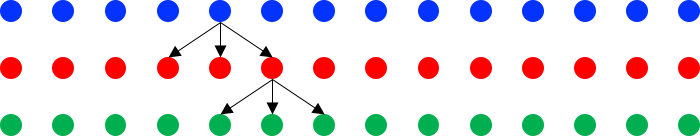
\includegraphics[height=0.5in]{TilingProcess/TilingProcess1.png}
		\caption{Original kernel iteration spaces and (abbreviated) dependences.}
		\label{tiling1}
	\end{subfigure}
	~~
	\begin{subfigure}[t]{0.45\columnwidth}
		\centering
		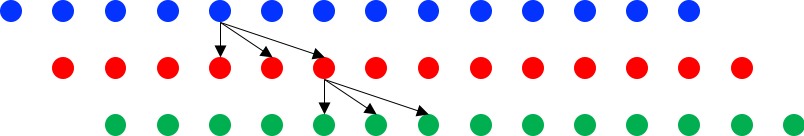
\includegraphics[height=.5in]{TilingProcess/TilingProcess2.png}
		\caption{After shifting kernels to remove negative dependences.}
		\label{tiling2}
	\end{subfigure}
	\par\bigskip
	\begin{subfigure}[t]{0.45\textwidth}
		\centering
		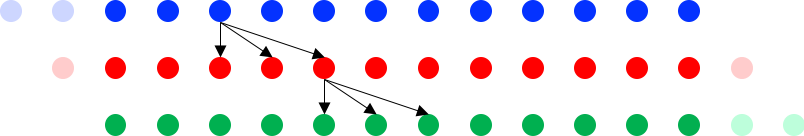
\includegraphics[height=0.5in]{TilingProcess/TilingProcess3.png}
		\caption{Shared iteration space. Chain could be fused sequentially.}
		\label{tiling3}
	\end{subfigure}
	~~
	\begin{subfigure}[t]{0.45\textwidth}
		\centering
		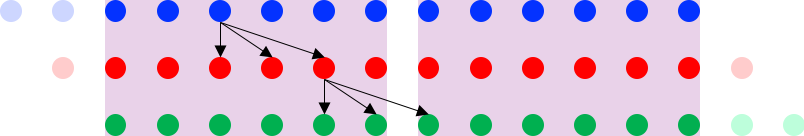
\includegraphics[height=.5in]{TilingProcess/TilingProcess4.png}
		\caption{Underlying tiles for TileSize=6 shaded in purple.}
		\label{tiling4}
	\end{subfigure}
	\par\bigskip
	\begin{subfigure}[t]{0.45\textwidth}
		\centering
		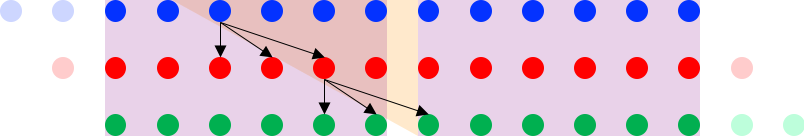
\includegraphics[height=0.5in]{TilingProcess/TilingProcess5.png}
		\caption{Overlap for each tile shaded in orange. Tiles against low edge have no overlap.}
	\end{subfigure}
	~~
	\begin{subfigure}[t]{0.45\textwidth}
		\centering
		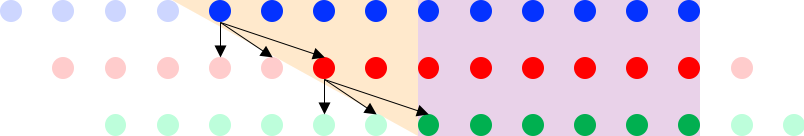
\includegraphics[height=.5in]{TilingProcess/TilingProcess6.png}
		\caption{An individual overlapped tile.}
	\end{subfigure}
	\par\bigskip
	\begin{subfigure}[t]{0.45\textwidth}
		\centering
		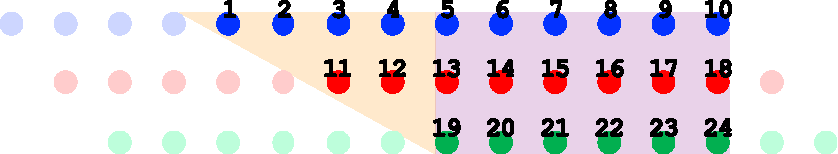
\includegraphics[height=0.5in]{TilingProcess/TilingProcess7.pdf}
		\caption{Execution order for an individual tile without fusion.}
		\label{tileNofuse}
	\end{subfigure}
	~~
	\begin{subfigure}[t]{0.45\textwidth}
		\centering
		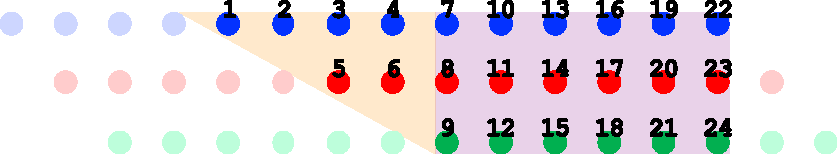
\includegraphics[height=0.5in]{TilingProcess/TilingProcess8.pdf}
		\caption{Execution order for an individual tile with fusion.}
		\label{tileFuse}
	\end{subfigure}
	\par\bigskip
	\begin{subfigure}[t]{\textwidth}
		\centering
		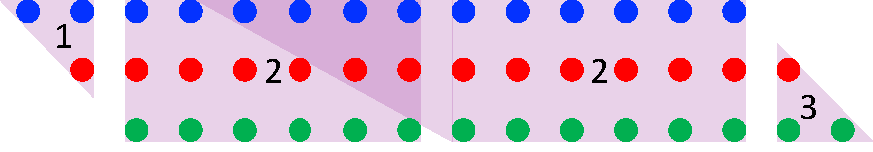
\includegraphics[height=0.5in]{TilingProcess/TilingProcess9.pdf}
		\caption{Global execution order for entire computation.}
		\label{tiling9}
	\end{subfigure}

\caption{Overlapped tiling of 3 one-dimensional loops.}
\label{tilingProcess}
\end{figure*}

\paragraph{Research Problems:}
The \verb.HYDRO_2D. benchmark shows significant data reuse across its three loops.
A loop transformation like overlapped tiling can leverage this reuse to improve performance.
However, because I have converted each loop one at a time, I have siloed the different stages of the computation, inhibiting any optimization across the stages.
Furthermore, because RAJA \verb.kernel. calls immediately execute the computation in question, I cannot perform any analysis or transformation beforehand.
This leads to a number of research questions:
\begin{itemize}
\item R1.1: How do we delay the execution of a computation so we can apply transformations?
\item R1.2: How can we best add an inter-loop context to RAJA to facilitate transformations like overlapped tiling?
\item R1.2: How do we check that transformations are safe to apply using information gathered only at runtime?
\item R1.4: How do we do this without sacrificing the performance improvements the transformations are meant to achieve?
\end{itemize}

\paragraph{Developed Solution:}


My approach has a number of components.
To address the need for a delay between the computation's description and execution, I introduced a wrapper object that holds the computation description until it is executed.
These wrapper objects are created by a function, \verb.make_kernel., with the same interface as the standard \verb.kernel. call. 
These kernel objects can be executed using the call operator.
Such an interface minimizes the code changes required to use it.
Listing~\ref{MakeKernelExample} shows how this function is used for the \verb.HYDRO_2D. case.

\begin{figure}
    \begin{lstlisting}[caption={Example usage of the \texttt{make\_kernel} function.},label={MakeKernelExample}]
//initialize segments and lambdas as above

//create kernel objects
auto knl1 = make_kernel<POL>(segment_tuple, lambda1);
auto knl2 = make_kernel<POL>(segment_tuple, lambda2);
auto knl3 = make_kernel<POL>(segment_tuple, lambda3);

//execute computation
knl1();
knl2();
knl3();
    \end{lstlisting}
\end{figure}

To address the need for an inter-loop context to facilitate transformations, I developed specialized functions for each transformation. 
Taking loop fusion as an example, the \verb.fuse. function takes a number of kernel objects as arguments and returns a new computation object that executes those kernels as a single fused computation. 

Lastly, to ensure the safety of the transformations, I introduced a symbolic evaluation system into RAJA.
This is where RAJA's View class comes into play. 
By overloading the View's call operator for a symbolic iterator type, I can gather access information without modifying any of the underlying data. 

%begin copy from rajalc paper

\begin{figure}
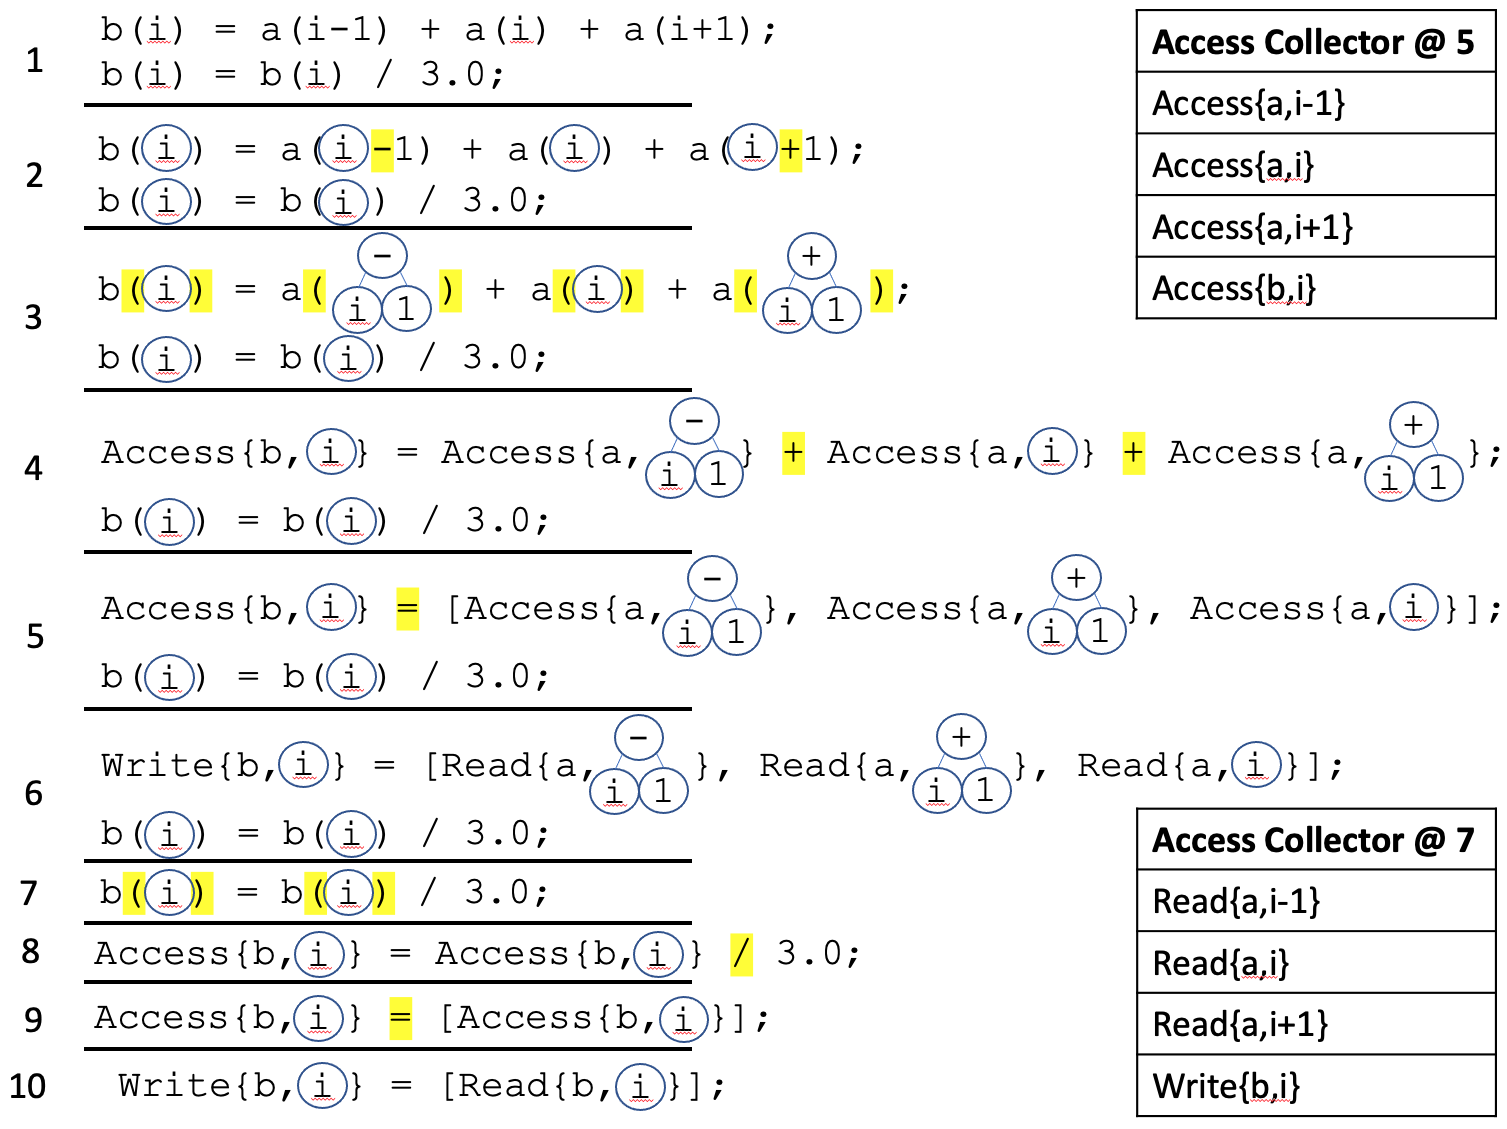
\includegraphics[width=\linewidth]{SymExecProcess.png}
\caption{Symbolic evaluation of a kernel lambda. 
Indexing expressions are evaluated first, then accesses, then statements in terms of accesses.
As assignments are evaluated, the accesses are marked as reads or writes.
Accesses are tracked using the access collector.}
\label{symExec}
\end{figure}

Figure~\ref{symExec} shows the process of symbolically evaluating the body of a lambda. 
We break kernel symbolic evaluation into two contexts: indexing and accessing. 
Indexing encompasses the representation and storage of index expressions, like
\verb.i+1. in \verb.a(i+1)..
The symbolic evaluation must retain the entire structure of the index expression 
because the loop's
data access pattern must reflect the difference between \verb.a(i+1). and
\verb.a(i-1)..
Indexing evaluation is shown in steps 2 and 3 of Figure~\ref{symExec}.
Accessing encompasses the statement-level data access semantics of the kernels.
Unlike with indexing, only whether accesses are reads or writes matters,
not the entire structure of the statements.
For example, we need to know that the statement \verb.c(i) = a(i) + b(i).
reads \verb.a(i). and \verb.b(i). and writes \verb.c(i)., but not that it
adds \verb.a(i). and \verb.b(i)..
Access evaluation is shown in steps 4, 5, and 6 of Figure~\ref{symExec}.
Listing~\ref{ExpressionGrammar} shows the grammar for supported indexing expressions and access statements. 
Behavior for kernels that do not use this grammar is undefined.

Normal RAJA kernel execution only affects the states of its Views. 
However, symbolic evaluation should not change View states. 
Instead, it should only preserve the access information.
We achieve this by adding a class-wide access collector to the symbolic iterator. 
When symbolic accesses are evaluated, they are added to the collector, and updated as reads or writes when assignments are evaluated.
This access collector and its contents at steps 5 and 7 are shown to the right in Figure~\ref{symExec}, and the change can be seen between steps 5 and 6.
 
\begin{figure}[t]
\begin{lstlisting}[label={ExpressionGrammar},caption={EBNF Grammar to Support Symbolic Evaluation}]
start : Access Assignment Expression
Expression : Expression Operator Operand | Operand
Operand : Access | Int | Double | Iterator
Operator : + | - | * | / | %
Assignment : = | Update
Update: += | -= | *= | /= | %=

Access : Id '(' IndexExpressions ')'
IndexExpressions : IndexExpression | IndexExpression ',' IndexExpressions
IndexExpression : IndexOperand Operator IndexExpression | IndexOperand
IndexOperand : Int | Double | Iterator
\end{lstlisting}
\end{figure}


\paragraph{Related Work:}

Bertolacci et al.~\cite{Bertolacci2016,Bertolacci2019} propose extensions to
OpenMP pragmas to express and schedule loop chains.
The approach requires annotations about data accesses in the pragmas.
That work enables the specification of loop fusion and wavefront tiling. 

Luporini et al.~\cite{Luporini2019} has a similar goal of enabling the source
code that uses a library  (in this case Devito~\cite{Luporini2018}) to
schedule across loop computations that share data.
The loops in their case have indirect array accesses.
Thus grouping computations to improve data locality requires a run-time
inspection phase~\cite{Strout14IPDPS}.
Luporini et al. use various Python library interfaces to specify computations
using per-loop modularization and then a lazy-computation step that gathers
the loop descriptions and generates inspector-executor code for performing 
sparse tiling.
The key differences between their work and ours is that we leverage the view 
capability of RAJA to avoid needing to annotate how data is being accessed
in each loop.  
Instead, our symbolic analysis collects that information.

\paragraph{Evaluation:}

Two metrics are used to evaluate this proposed research: performance improvement and code delta. 
For both metrics, I look at three variants of each evaluated code.
The first variant is the original RAJA implementation. 
The second variant is the original RAJA implementation, modified to implement the transformation by hand.
The third variant implements the transformation using my contribution.

I look at the execution time for single-node executions, comparing the execution times among the three variants. My contribution provides slightly lower performance improvements than the hand-implemented variant, due to overhead of the system.

I also compare the difference in the source lines of code changed to implement each variant.

\paragraph{Preliminary Results:}
Evaluation results indicate a similar performance improvement to hand-implementation with significantly fewer code changes.
Figure~\ref{RAJAPerfPerf} shows the change in performance for benchmark kernels optimized by hand (blue) and with RAJALC (green). 
Table~\ref{sloc} shows the source lines of code changed and added for the different implementations of the benchmark programs.

\begin{figure}
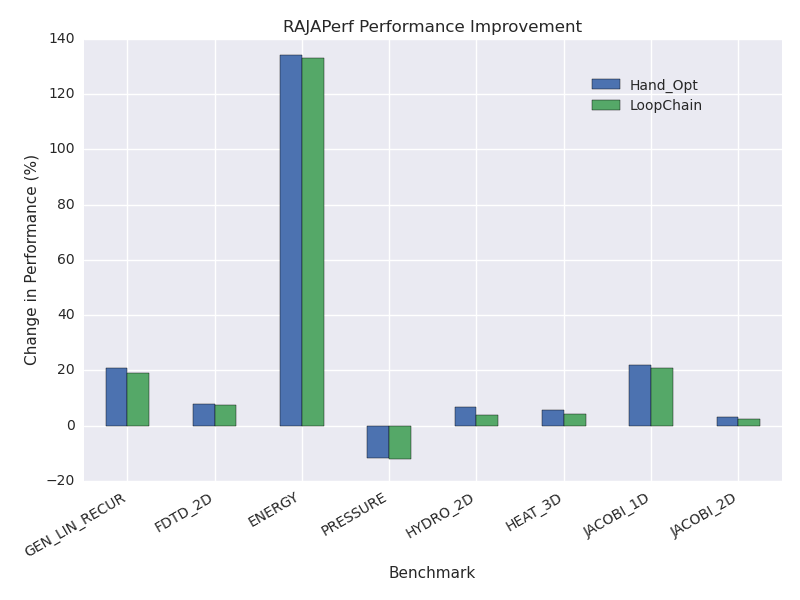
\includegraphics[width=0.5\textwidth]{RAJALC-perf-system-1.png}
\caption{Performance changes of RAJAPerf benchmarks on System Intel1 (higher is better).}
\label{RAJAPerfPerf}
\end{figure}


\begin{table}[t]
    \begin{tabular}{|l|l|l|l|l|}
    \hline
    \textbf{Benchmark}       & \multicolumn{2}{l|}{\textbf{\begin{tabular}[c]{@{}l@{}}Manual \\ Implementation\end{tabular}}} & \multicolumn{2}{l|}{\textbf{\begin{tabular}[c]{@{}l@{}}RAJALC\\ Implementation\end{tabular}}} \\ \hline
    \cellcolor[HTML]{9B9B9B} & Changed                                         & Added                                        & Changed                                        & Added                                        \\ \hline
    \textit{ENERGY}          & 6                                               & 6                                            & 6                                              & 2                                            \\
    \textit{PRESSURE}        & 2                                               & 3                                            & 2                                              & 2                                            \\
    \textit{GEN\_LIN\_RECUR} & 1                                               & 1                                            & 2                                              & 2                                            \\
    \textit{FDTD\_2D}        & 8                                               & 4                                            & 9                                              & 4                                            \\
    \textit{HYDRO\_2D}       & 4                                               & 41                                           & 3                                              & 2                                            \\
    \textit{JACOBI\_1D}      & 3                                               & 17                                           & 3                                              & 3                                            \\
    \textit{JACOBI\_2D}      & 10                                              & 33                                           & 10                                             & 3                                            
    \\
    \textit{HEAT\_3D}        & 12                                              & 38                                           & 12                                             & 3                                            \\ \hline
    \textit{Average}        & 5.8                                              & 17.9                                           & 5.9                                            & 2.6                                            \\ \hline
    %\textit{Average}        & 5.75                                              & 17.875                                           & 5.875                                            & 2.625                                            \\ \hline
    \end{tabular}
    \caption{Lines of Code Impact to implement transformations by hand and with RAJALC.}\label{sloc}
    \end{table}


\subsection{Work in Progress: Data Transformations in RAJA}
\label{Sec:Work2}
The layout of data in memory is a key consideration in high performance computing applications.
From reducing cache and page misses to relieving pressure on memory bandwidth and avoiding inter-process communication, using a good data layout improves performance at all levels of an application.
RAJA's Views incorporate data layout as part of their initialization, allowing a user to try out different layouts without major refactoring costs.
However, some applications benefit from changing the data layout mid-computation to facilitate better locality.
Implementing such a mid-computation layout change in RAJA can improve performance, but is laborious to implement and lacks portability.
Thus, I propose introducing a lightweight, declarative API for changing data layouts between computations.
Furthermore, I propose developing a performance model for layouts using the loop bounds and data access order as input and a runtime interface that dynamically estimates performance to select an appropriate layout. 
These systems combine so that the model and runtime \enquote{fill in} layout choices that the user did not specify.

\paragraph{Context and Background:}

Figure~\ref{DataLayoutImportance} shows the importance of a good data layout. 
The BadLayout column shows the execution time for a matrix multiplication where the three arrays are laid out opposite of their access order. 
The GoodLayout column shows the execution time for the same matrix multiplication when the arrays are laid out to match their access order.
The LayoutChange column shows the execution time of code that changes the layout from the bad layout to the good one.
Finally, the SwitchAndRun column shows the combined execution time of changing the layout from bad to good and then running.
As the graph shows, performance improves  significantly (72\%) simply by changing the data layout, and the cost of performing the layout change is small (<1\% of execution time). 

General purpose libraries like Kokkos and RAJA and programming languages like Chapel~\cite{diaconescu2007approach} give programmers some control over the data layout of multi-dimensional arrays. However, this support is limited to the point of initialization.
Thus, programmers must use that particular data format for the entire computation.
While a developer could change the data layout mid-computation in RAJA, the developer must either modify RAJA library code or use multiple arrays for the same data. 
Both options increase the code complexity and increase its fragility.
The brave developer who chooses one of these options must still overcome yet another obstacle: selecting the right combination of formats.
Even a modest computation of two loops that use four 2D arrays has more than 200 combinations from which to choose, so trying all possible options quickly becomes infeasible. 

A significant body of work has developed Integer Linear Programming (ILP) formulations to determine data layouts in distributed memory settings for programming languages like HPF and D~\cite{bixby1994automatic,kennedy1995automatic,kennedy1998automatic}. 
A similar line of work~\cite{chen2004ilp,chen2005constraint,chen2005integrating, ozturk2011data} uses ILP-based constraint networks to combine data layout and schedule optimizations. 
Both approaches were developed in the context of a compiler. 
We build on an important idea from them: use a performance model encoded as the objective function in an ILP problem to automate data layout decisions (partially or fully).
Rather than only applying this data layout compiler technology automatically, we provide it to the user through a library interface while still enabling its automated use.
Our library and runtime approach allows the user to guide use of the technology to focus on loops most likely to benefit from it.
However, the library must perform its analysis and decision making at runtime and the interface must be high-level while still providing enough control. 
These challenges lead to a number of sub-problems such as interface design so that the analysis cost is low (enough) while maintaining ease of use.
A compiler approach can take longer and has all information that the language semantics provide.
Some advantages of a library approach are that it is more accessible to users and the library implementation will have more information available, such as loop bounds, accessible at runtime before a loop executes.
Although useful advantages, these lead to further sub-problems about how the library implementation can most leverage the compiler of the language in which it is embedded (C++ here) to force as much specialization as possible to achieve the ultimate goal of performance.
\begin{figure}
	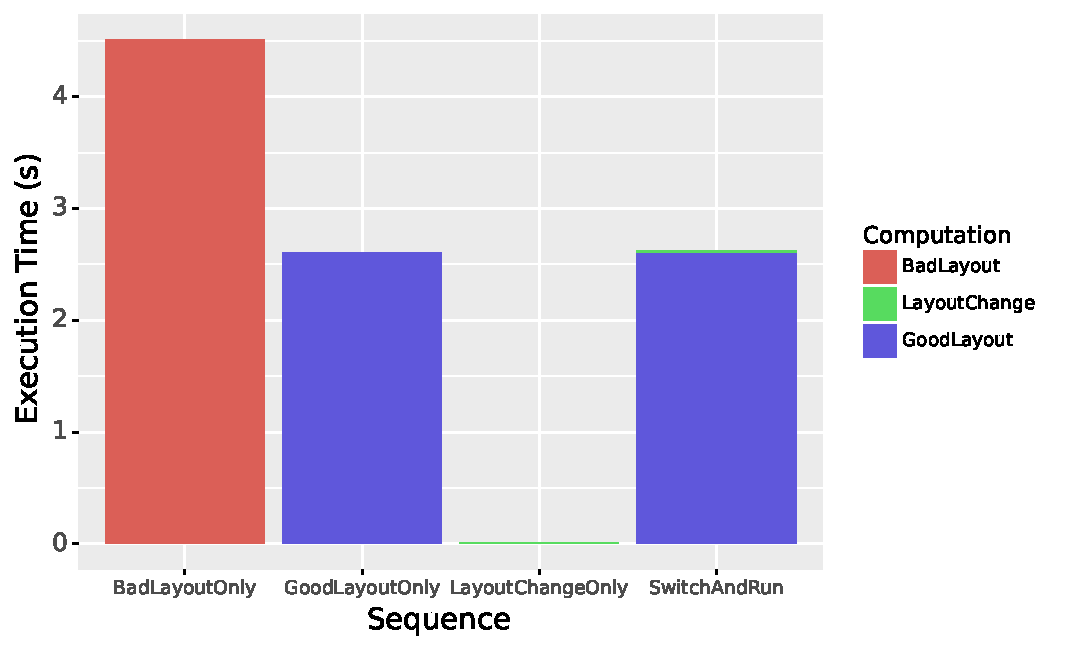
\includegraphics[width=\columnwidth]{IntroExampleGraph.pdf}
	\caption{Execution time for matrix multiplication using optimal and non-optimal data layouts and execution time for converting from non-optimal to optimal.}
	\label{DataLayoutImportance}
	%\Description[Matrix Multiplication Execution Time for Different Layouts]{A bar plot showing a "Bad Layout" column with execution time greater than the "Good Layout" and "Layout Conversion" columns combined.}
\end{figure}



\paragraph{Research Problems:}

\begin{itemize}
\item R2.1 How do we expose layout transformation specification to the user ergonomically?
\item R2.2 How do we accurately and efficiently estimate the cost of making different layout changes?
\item R2.3 How do we minimize the runtime overhead of solving the ILP formulation?
\end{itemize}

\paragraph{Proposed Solution:}

I propose developing a declarative API for changing data layout between kernels, and an ILP model for making additional data layout choices.
Listing~\ref{FormatDecisions3MM} shows how the 3MM benchmark would be implemented using my proposed API. 
The new \verb.FormatDecisions. object is the central component of our system. 
Its instantiation, using the \verb.format_decisions. function, takes a tuple of references to Views that are possible targets of format changes and the kernel objects that constitute the whole computation.
Two methods are used to register desired formats: \verb.set_format_before. and \verb.set_format_after..
Both take the View to be reformatted, the desired format, and the computation before or after which the desired format should be used.
Once all format choices are registered, the complete computation with the desired format conversions is generated using the \verb.finalize. method.

\begin{figure}
\begin{lstlisting}[caption={The 3MM benchmark implemented using FormatDecisions.},
    label={FormatDecisions3MM}]
auto knl1 = make_kernel<KPOL>(segs1, [=](auto i0, auto i1, auto i2) {
    E(i0, i1) += A(i0, i2) * B(i2, i1);
});
auto knl2 = make_kernel<KPOL>(segs2, [=](auto i0, auto i1, auto i2) {
    F(i0, i1) += C(i0, i2) * D(i2, i1);
});
auto knl3 = make_kernel<KPOL>(segs3, [=](auto i0, auto i1, auto i2) {
    G(i0, i1) += E(i0, i2) * F(i2, i1);
});

auto decisions = format_decisions(tie(B,D,F), knl1, knl2, knl3);

decisions.set_format_before(B, {{1,0}}, knl1);
decisions.set_format_before(D, {{1,0}}, knl2);

decisions.set_format_before(F, {{0,1}}, knl1);
decisions.set_format_after(F, {{1,0}}, knl2);

auto computation = decisions.finalize();
computation();
\end{lstlisting}
\end{figure}

For the ILP model, I use binary decision variables representing whether or not a particular format is used at different points in the chain. 
For example, there are eight decision variables for the \verb.B. View in Listing~\ref{FormatDecisions3MM}, one for each of the two possible formats at each of the four points in the chain. 
While there are only three kernels in the chain, there is an additional point added for the \enquote{output} format that the View has after the computation is done.

Symbolically, we represent the variables as follows.
To start, let $F$, $K$, and $T$ represent the set of all formats, kernels, and conversion times.
Because we add additional elements to $K$ for the input and output formats, we know that $|K|$ is the number of user kernels plus 2.
Furthermore, because there is one more conversion than kernel, we know that $|T| = |K| + 1$.
For each kernel, we have one variable for each format. 
Thus, let $fmt_{f,k}$ denote the variable for using the format $f$ during kernel $k$, where $f \in F$ and $k \in K$.
For conversion variables, we have one variable for each possible conversion at each time point. 
Thus, let $conv_{i,o,t}$ denote the decision variable for converting from format $i$ to to format $o$ at conversion time $t$, where $i,o \in F$ and $t \in T$.

Four types of constraints are imposed on the decision variables.
\begin{itemize}
\item Format Uniqueness: At each time point, the View has exactly one selected format. Given by: 
\begin{align*}
	\bigwedge\limits_{k \in K} (1 = \sum\limits_{f \in F} fmt_{f,k})
\end{align*}
\item Conversion Uniqueness: At each conversion point, the View goes through exactly one conversion. Given by:
\begin{align*}
	\bigwedge\limits_{t \in T} (1 = \sum\limits_{i \in F}\sum\limits_{o \in F} conv_{i,o,t})
\end{align*}
\item Format-Conversion Matching, Input: At each conversion point, the input format for the conversion matches the format of the preceding kernel. Given by:
\begin{align*}
	\bigwedge\limits_{t \in T} \bigwedge\limits_{i \in F} fmt_{i,t.prev} = \sum\limits_{o \in F} conv_{i,o,t}
\end{align*}
\item Format-Conversion Matching, Output: At each conversion point, the output format for the conversion matches the format of the following kernel. Given by:
\begin{align*}
	\bigwedge\limits_{t \in T} \bigwedge\limits_{o \in F} fmt_{o,t.next} = \sum\limits_{i \in F} conv_{i,o,t}
\end{align*}
\item User Prescription: All user-provided format choices are met. With all user choices $U$ represented as pairs of a kernel and the format the user wants for that kernel, given by:
\begin{align*}
	\bigwedge\limits_{(k,f) \in U}  fmt_{f,k} = 1
\end{align*}
\end{itemize}


\paragraph{Evalution:}

I will perform a similar evaluation to the loop schedule optimization proposal, looking at source lines of code added, removed, or modified; and changes in execution time among the different variants.


\paragraph{Preliminary Results:}

Preliminary results indicate that while there is performance improvement available through layout transformations, modelling which layouts to choose introduces more overhead than performance improvement. 


\paragraph{Summary of Reviewer Critiques:}

This work was submitted for peer review at the International Conference on Supercomputing 2022 (ICS2022). 
While praised for its clear writing and \enquote{elegant} approach to reducing programmer intervention, it was ultimitely rejected.
The key elements the reviewers found lacking were:
\begin{itemize}
\item Minimal evaluation (4 benchmarks, only 2 show improvement, and no full applications)
\item Limited to loops with perfect loop nests
\item Limited discussion of related work
\end{itemize}
I will expand evaluation to include more benchmarks and at least one full application, expand on the related work to place my work in context (current progress immediately following), and expand support to imperfectly nested loops. I will also develop more techniques for reducing the modelling overhead.

\paragraph{Related Work}
Early approaches to optimizing data locality use schedule transformations rather than data layout transformations. 
Work incorporated into the SUIF compiler uses interchange, reversal, skewing, and tiling~\cite{wolf1991data}, whereas Fortran source-to-source approaches also use loop fusion~\cite{mckinley1996improving}.
While schedule transformations avoid the overhead cost of layout conversion, their global nature can improve locality for one access while harming another.
Nevertheless, schedule transformations remain a popular approach to optimizing data locality and parallelism, 
especially through tiling techniques~\cite{bondhugula2008pluto,bertolacci2015parameterized,bondhugula2016diamond,bandishti2012tiling,unat2016tida}.

In the domain of data layout transformations, early work in High Performance Fortran (HPF) and D compilers~\cite{bixby1994automatic,kennedy1995automatic,kennedy1998automatic} provide foundations for a variety of later approaches.
Their framework follows a popular pattern: generate a space of possible choices, estimate the performance of different choices, and select an option using an ILP formulation. 
My ILP problem formulation is similar to theirs, although we do not use the data layout graph intermediate representation.
Furthermore, where their model for cost estimation focuses on communication costs in a distributed context, my approach models on-node performance costs of cache misses.

The polyhedral model, traditionally used for schedule transformations, is commonly leveraged for data layout transformations as well.
With the rise of multicore chips, new strategies were needed to manage shared on-chip resources. 
Work by Lu et al.~\cite{lu2009data} and Zhang et al.~\cite{zhang2011optimizing} develop layout optimization schemes based on the polyhedral model and use a combination of strip-mining, permutation, and padding transformations.


Data layout transformation frameworks are also popular for heterogeneous programming systems, especially for stencil codes.
Sung, Stratton, and Hwu~\cite{sung2010data} use data layout transformations to relieve pressure on memory controllers in structured grid applications by spreading data out across the address space based on the indexing behavior of the application.
Henretty et al.~\cite{henretty2011data} develop a layout transformation and accompanying static analysis to address stream alignment conflicts for SIMD architectures.
Jaeger and Barthou~\cite{jaeger2012automatic} present a strategy for generating stencil codes with optimal data layouts using a multi-padding layout transformation.
Recognizing the need for specialized support for ever-changing chip structure, Majeti et al.~\cite{majeti2013compiler} develop a programmer (or autotuner) guided data transformation system.
Built into the Habenero-C compiler, the meta-data provided by the user guides the generation of architecture-specific SOA, AOS, and SOAOS data layouts.
Another approach by Kofler, Cosenza, and Fahringer~\cite{kofler2015automatic} convert AOS implementations to other data layouts for GPU applications automatically.  
With the exception of Majeti et al., these approaches do not provide an interface to the developer, and without exception are compiler-based approaches.
My approach presents an interface to the developer in the form of a library API, allowing user control and low-cost integration into existing workloads.

Although still in the realm of the compiler-based tecniques, pragmas have been suggested as a solution to the problem of providing control over the transformations to the user.
Proposals to add such pragmas have been submitted to OpenMP~\cite{kruse2019design} and Clang~\cite{kruse2018user}.
Other work has implemented transformation pragmas into a source-to-source compiler~\cite{xu2014semi}. 


Domain-specific language approaches are another avenue for presenting users with control of the data layout transformations to apply. 
Kronawitter et al.~\cite{kronawitter2018automatic} incorporate data layout specifications into the ExaSlang DSL.
Using a polyhedral framework, the Tiramisu DSL~\cite{baghdadi2019tiramisu} also enables data layout transformation specifications.
In constrast to these specialized approaches, my approach seeks to support a wider class of computations without needing the additional machinery required to use DSLs. 


\subsection{Proposed Research: Sparse Data Formats in RAJA}
\label{Sec:Work3}
Computations on sparse data are widespread. 
For example, any simulation using unstructured meshes require some sort of sparse representation.
While RAJA effectively separates concerns for dense codes, this is lost for sparse codes.
\todo{indicate why this is a probleM}
For instance, consider how data is indexed when using compressed sparse row (CSR). 
The data format is baked directly into the description of the computation, so changing the format of the data requires extensive refactoring of all parts of the kernel.
I propose extending RAJA's separation of concerns into the domain of sparse codes to enable the portable description of computations on sparse data.

\paragraph{Context and Background:}
\begin{figure}
\begin{lstlisting}[caption={CSR-stored sparse matrix vector multiplication},label={SpMVCSR}]
for(i = 0; i < N; i++) {
    y(i) = 0;
    for(j = A.rowptr(i); j < A.rowptr(i+1); j++) {
        y(j) = y(j) + A.val(j) * x(A.col(j));
    }
}
\end{lstlisting}
\end{figure}

A common kernel within sparse codes is the multiplication of a sparse matrix $A$ with a dense vector $x$.
Listing~\ref{SpMVCSR} shows how part of such a code is implemented when $A$ is stored using compressed sparse row.
These six lines elucidate how thoroughly intertwined the implementation is with the format of the sparse matrix $A$.
Note that even the accesses to $y$, ostensibly unconnected to $A$, are still based on values within $A$'s row pointer.
A developer seeking to change the storage format of $A$ must change almost the entire loop nest, a highly unscalable solution.

Existing approaches, such as the Tensor Algebra Compiler (Taco)~\cite{kjolstad2017tensor}, can portably represent SpMV and change the storage formats, but are restricted to computations with only reduction dependences.
This excludes common computations like direct solve.

No matter the system used to represent the computation, the importance of good layout choice is even greater for sparse computations.
While memory hierarchy means there are some benefits to be found in dense codes, dense arrays are constant time accessible ($O(1)$), so performance benefits come from a reduction of that nebulous constant $M$.
For CSR data, a poorly scheduled traversal can require a search for each access.
This means that proper format and schedule choice can reduce the algorithmic complexity of the computation.


\paragraph{Research Problems:}
\begin{itemize}
    \item R3.1: How do we extend the decoupling of data, operation, iteration space, and schedule description into the sparse context while maintaining idiomatically RAJA-like code?
    \item R3.2: How do we formulate format selection for sparse codes as an ILP problem?
    \item R3.3: How do we efficiently estimate the cost of choosing different sparse formats?
    \item R3.4: How do we support efficient iteration through sparse data without the ability to rewrite the operation for a particular format? 
\end{itemize}


\paragraph{Proposed Solution:}


\begin{figure}
\begin{lstlisting}[label={ForwardSolveC},caption={C-like implementation of forward substitution using Views}]
View2D A(N,N);
View1D x(N);
View1D b(N);

/* copy b into x */

for(int i = 0; i < N; i++) {
    for(int j = 0; j < i; j++) {
        x(i) = x(i) - A(i,j) * x(j);
    }
}
\end{lstlisting}
\end{figure}


\begin{figure}
\begin{lstlisting}[caption={Possible RAJA implementation of forward substitution.},label={ForwardSolveRAJA}]
auto lam = [&](auto i, auto j) {
    //note that references to A are format-independent
    x(i) = x(i) - A(i,j) * x(j);
};

using POL = KernelPolicy<
    statement::For<0,loop_exec,
        statement::For<1,loop_exec,
            statement::Lambda<0>
        >
    >
>;

auto seg0 = A.nonzeros(0);
auto seg1 = A.nonzeros(1) && RangeSegment(0,seg0.val());

auto segs = make_tuple(seg1, seg2);

auto knl = make_kernel<POL>(segs, lam);

auto chain = make_chain(knl);

//set the data format for A during knl
chain.set_data_format(knl,A,Format::CSR);

chain();

\end{lstlisting}
\end{figure}

The problem of decoupling has, ironically, a number of interrelated components.
First, what does it mean for code to be \enquote{idiomatically RAJA-like?}
I use a rather subjective notion: that a programmer familiar with RAJA recognizes the structure and semantics of the code. 
To achieve this, the description of a sparse computation should look as much like a dense code as possible. 

With this in mind, I turn to each component of the computation.
Starting with the previously mentioned coupling of the data format and operation, I recognize that through using Views, we already have a format-agnostic method for describing the computation. 
Thus, the lambdas should be written as if they were operating on dense Views, and all format specific indexing behavior should be abstracted into the View class itself. 
I suggest a similar approach for the schedule description as well.

The iteration space description requires more modification, illustrated by an example.
Listing~\ref{ForwardSolveC} shows a C-like implementation of the forward substitution step in a direct solve of the linear system $Ax=b$, a common kernel in sparse codes.
When $A$ is sparse, we do not need to iterate through all values in the dense iteration space.
Instead, we only need to iterate over the points where $A$ is nonzero. 
Thus, we need a way of reducing the iteration space to only the necessary points. 
I propose a symbolic iteration description API.
Views will have a method \verb.nonzeros(i). that represent the non-zero index values of the $i$th dimension. 
Segment dimensions will have a method \verb.value(). that represents the current value of that iterator, allowing for triangular and other shaped iteration spaces.
Finally, operator overloading will allow for the combination multiple ranges.
Line 15 of Listing~\ref{ForwardSolveRAJA} shows how this overloading could be used to combine the nonzero condition with the $j < i$ condition.

I now pivot to the problem of efficient iteration of the data.
Existing approaches to representing and optimizing sparse codes, such as Taco and the Sparse Polyhedral Farmework (SPF)~\cite{strout2016approach}, have an important feature that my proposed work does not: they are compilers.
While this adds complexity to the toolchain, it enables these approaches to perform rewriting steps based on the sparse format.
Thus, they can rewrite the access \verb.A(i,j). as some expression calculating a \verb.val_index. and then replacing the access to \verb.A. with \verb.val[val_index]..
In contrast, my proposed approach is incorporated into RAJA using only standard C++ features and compilers (GCC/Clang).
Because loop bodies in RAJA are specified as lambda closures, we cannot rewrite (or even directly inspect) the operations they perform.

To address this challenge, I lean on the wealth of information known about the computation, specifically the execution schedule provided by the user and the access information collected through symbolic evaluation. 
First, as part of the definition of a sparse format, one or more \enquote{efficient traversal orders} are declared. 
For example, CSR would have $(0,1)$ as a efficient traversal order, while CSC would have $(1,0)$.
Second, before the computation is executed, each sparse View in the computation will be prepared for the computation that is about to execute.
This preparation will change the backend behavior of the call operator.
If the computation is traversing the View's data in one of the specified efficient orders, the access function will guide the traversal through the data in an efficient manner.
Otherwise, the access function will perform the default behavior for the format, likely involving searching the index structure of the View.
Listing~\ref{BackendSketch} sketches some of these components for the CSR format. 

\begin{figure}
\begin{lstlisting}[caption={Sketch of the backend for efficient iteration}, label={BackendSketch}]
View::prepare_for_traversal(Schedule schedule, SymAcess accessInfo) {
    auto traversalOrder = simplify(schedule, accessInfo);

    if(this->traversalFunctions.contains(traversalOrder)) {
        this->access_function = efficientTraversals[traversalOrder];
    } else {
        this->access_function = standard_access;
    }
}

CSR::standard_access(Index i0, Index i1) {
    auto col_lo = rowptr[i0];
    auto col_hi = rowptr[i0+1];
    auto val_index = search(col,col_lo, col_hi, i1);
    if(val_index != -1) {
        return val[val_index];
    }
}


CSR::efficient_traversal_access(Index i0, Index i1) {
    auto val_index = -1;
    if(last_i0 == i0) {
        val_index = last_val_index;
    } else {
        val_index = rowptr[i0];
    }

    while(col[val_index] != i1 && val_index < rowptr[i0+1]) {
        val_index += 1;
    }

    last_val_index = val_index;
    last_i0 = i0;
    last_i1 = i1;
    if(col[val_index] == i1) {
        return val[val_index];
    } else {
        return 0;
    }
}

CSR::efficientTraversals[[0,1]] = CSR::efficient_traversal_access;
\end{lstlisting}
\end{figure}

Another possible approach may be to attempt to simulate the rewriting of the lambda based on the symbolic evaluation results by translating the symbolic evaluation result into a format-specific access.
However, this is likely highly ineffecient, and may be obstructed by lambda type requirements.


\begin{figure}
\begin{lstlisting}[caption={Possible RAJA implementation of Sparse Matrix Multiply.}, label={SparseMMRaja}]
    
auto lam = [&](auto i, auto j, auto k) {
    C(i,j) += A(i,k) * B(k,j);
}
using POL = KernelPolicy<
    statement::For<0,loop_exec,
        statement::For<1,loop_exec,
            statement::For<2,loop_exec,
                statement::Lambda<0>
            >
        >
    >
>;

auto seg1 = A.nonzeros(0);
auto seg2 = B.nonzeros(1);
auto seg3 = A.nonzeros(1) * B.nonzeros(0);
auto segs = make_tuple(seg1,seg2,seg3);

auto knl = make_kernel<POL>(lam,segs);

auto chain = make_chain(knl);

chain.set_data_format(knl,A,Format::CSR);
chain.set_data_format(knl,B,Format::CSC);
chain.set_data_format(knl,C,Format::COO);

chain();

\end{lstlisting}
\end{figure}

Finally, I turn to the problem of formulating format selection as an ILP problem and cost estimation.
My planned approach is somewhat similar to that presented in Section~\ref{Sec:Work2} for use with dense codes.
However, there are some important differences. 
First is the potential to reduce the algorithmic complexity of the computation. 
This suggests that dynamic cost estimation via small benchmarks may not be best for capturing the potential costs.
Ahrens, Kjolstad, and Amarasinghe~\cite{ahrens2021asymptotic} present a related approach to selecting schedules for sparse programs, and their cost modelling approach may be useful in selecting formats.
The other major difference is the influence of the data's sparsity on the performance results. 
This will have to be incorporated into the model to accurately estimate the benefit of format changes.



\paragraph{Related Work}

A number of works provide frameworks for describing different sparse data formats. 
Ahmed et al.~\cite{ahmed2000framework} presents a combined framework for describing sparse matrix indexing structures and generating sparse implementations from dense computation descriptions.
In their framework, sparse formats are described in terms of the relationship between different dimensions. For example, CSR has the index structure $r \rightarrow c \rightarrow v$, indicating rows must be accessed first, then the columns and values can be enumerated.
ADditionally, each dimension of the representation can be annotated with information about the enumeration order (random-access, increasing-order-only, etc.) and the enumeration bounds (triangularity).
The implementation of this framework is described in more detail in~\cite{mateev2000next}.
A key concept in this framework is having a random access view of the data for algorithm writers and a sequential access view for the compiler.
The compiler can then use the sequential access logic when the computation allows and can fall back on the random-access logic if necessary. 
My approach uses a similar multi-logic access.

Chou, Kjolstad, and Amarasinghe~\cite{chou2018format} describe an alternative framework for describing sparse formats in the context of tensor algebra. 
In this framework, sparse formats are broken into individual dimensions which have one of six level formats. 
These level formats each have traversal logic that enable the generation of arbitrary iteration code for the format.
In contrast to my proposed approach, this framework relies heavily on a code generation step, as it is a component of Taco.

Popoola~\nc presents an approach for generating code for converting between different sparse formats.
Based on the Sparse Polyhedral Framework~\cite{strout2018sparse}, sparse formats are described using a number of relations between data and indices. 
By composing relations that use the dense format as an intermediary, Popoola generates efficient transformations between arbitrary sparse formats.


\todo{libraries}




\todo{augustine2019}



Taichi~\cite{hu2019taichi} is a programming language for spatially sparse (globally sparse, locally dense) computations.
Embedded into C++, computations are expressed as format-agnostic kernels, which are then optionally annotated with optimizations.
Then, the Taichi compiler lowers the frontend code to an intermediate representation and finally to standard C++ or CUDA code. 
Then, this generated code is compiled using a standard C++ compiler.
In contrast, my approach is wholly contained within standard C++, avoiding the need to add additional configuration, building, or linking.
\todo{How taichi does format description}








\begin{table}
\begin{tabular}{|c|c|c|c|}
\hline
Approach & Format-agnostic representation & Tensor expressions & Arbitrary dependences \\
\hline
Taco~\cite{kjolstad2017tensor} & \yes & \yes & \no \\
Taichi~\cite{hu2019taichi} & \yes & \yes & \yes \\
\cite{ahmed2000framework} & \yes & \yes & \yes \\ 
My Approach & & & 
    
\end{tabular}
\caption{Table of capabilities for different approaches}
\label{MagicTable}
\end{table}


% \subsection{Complete Example}

% Start with the SpMM implementation from Listing~\ref{SparseMMRaja}.
% This subsection will walk through my proposed approach step by step.
% First, I will show how the model selects a data format. 
% Then, I will show how the selected data format is applied to each View.

% Before we start, I restrict the problem to N-dimensional compressed sparse fiber, with arbitray dimension ordering. 
% In this restricted problem, compressed sparse row (CSR) is \verb.Format::CSF(0,1). and compressed sparse column (CSC) is  \verb.Format::CSF(1,0).

% \paragraph{Format Model:}
% This example's model has four values to identify:
% \begin{itemize}
%     \item Data format for A
%     \item Data format for B
%     \item Data format for C
%     \item Execution nesting order
% \end{itemize}
% Generally, for each kernel in a chain, we model variables for each View's data format and the execution nesting order for that loop nest.


% For the execution nesting order, the model will not be able to use different execution nesting orders, because the order is provided as a template argument. 
% However, the system will be able to alert the programmer that there is a potentially better order choice.

% Let's enumerate every variable in the model and what it's name indicates. 
% \begin{itemize}
%     \item \verb.A_fmt_0_1. True if A's format is ordering $(0,1)$, false otherwise
%     \item \verb.A_fmt_1_0. True if A's format is ordering $(1,0)$, fales otherwise
%     \item \verb.B_fmt_0_1. True if B's format is ordering $(0,1)$, false otherwise
%     \item \verb.B_fmt_1_0. True if B's format is ordering $(1,0)$, fales otherwise
%     \item \verb.C_fmt_0_1. True if C's format is ordering $(0,1)$, false otherwise
%     \item \verb.C_fmt_1_0. True if C's format is ordering $(1,0)$, fales otherwise
%     \item \verb.nest_0_1_2. True if the nesting order is $(0,1,2)$, false otherwise
%     \item \verb.nest_0_2_1. True if the nesting order is $(0,2,1)$, false otherwise
%     \item \verb.nest_1_0_2. True if the nesting order is $(1,0,2)$, false otherwise
%     \item \verb.nest_1_2_0. True if the nesting order is $(1,2,0)$, false otherwise
%     \item \verb.nest_2_0_1. True if the nesting order is $(2,0,1)$, false otherwise
%     \item \verb.nest_2_1_0. True if the nesting order is $(2,1,0)$, false otherwise
% \end{itemize}

% Now let's consider the constraints on these variables. 
% First, we have constraints so that there is only one format per View per computation. For A, this constraint looks like \verb.A_fmt_0_1 + A_fmt_1_0 = 1..
% A similar approach generates constraints for nesting variables
% \todo{format translation variables}

% Finally, I need to describe the terms in the objective function.
% I need to take into account the interaction between the variables in the model.
% I assume there is only interaction between data format variables and nesting order variables. 
% This means that for each combination of format variable and schedule variable, I run a dynamic microbenchmark accessing data with the format using the particular schedule. 
% For the combo of \verb.A_fmt_0_1. and \verb.nest_0_1_2., let the execution time of the microbenchmark be \verb.ExecTime.
% Further, let \verb.A_size. be the size of A. 
% Then the term in the objective function will be \verb.(ExecTime * A_size) * A_fmt_0_1 * nest_0_1_2..

% There will also need to be objective function terms for the cost of translating from one format to another. 

% \paragraph{Applying the Format}
% Once a format is selected, I need to propogate that format into the Views. 
% This problem is tied with how the accesses are made efficiently. 

\section{Limitations}
\label{Sec:Limitations}
One self-imposed limitation of my proposal is the space of sparse formats I will support.
Because I focus on CSF, Coordinate, and Dense formats, codes that use formats outside of this space will not be able to use my framework.
More broadly, the impact of this work is partially limited by the host library RAJA. 
However, a similar approach could be used in other libraries like Kokkos, or libraries for different languages all together.

Another limitation of my work is that it does not support doing data and schedule transformations at the same. 
There is ample evidence that co-optimizing schedule and layout provides more performance improvement than either on their own \todo{cite Vivek's paper on this}. 
Similarly, support for more transformations, like wavefront parallelism scheduling and AoS-SoA conversions would expand the class of applications that my contribution could be used for.

Finally, because of the heavy templating involved in my approach, error messages can be difficult to decipher. 
This is a familiar problem \todo{cite the papers from the EDSL class}, but its solution is out of the scope of this work.


\section{Project Schedule}
\label{Sec:Schedule}
I set out the following schedule for my dissertation research.

\subsection{Data Layout Transformation Paper Resubmission}

\paragraph{Task:} I will improve my ICS2022 paper for resubmission at either LCPC (likely July/August) or OOPSLA (likely October). 
The improvements I will make are a better discussion of related work, evaluation on a complete application rather than only benchmarks, evaluation on multiple machines, and reduction of the modeling overhead.
This submission will answer my research questions about exposing layout transformation specification, accurate and efficient estimation of layout change cost, and overhead minimization for solving the ILP formulation.

\paragraph{Deliverable, Summer/Fall 2022:} Revised and submitted paper.


\subsection{Evaluation Kernel Collection}

\paragraph{Task:} I will curate example computations for the evaluation of my contribution.
These computations will exhibit a variety of access patterns, dependence patterns, and data sparsity.
Each computation will be paired with input data representative of their source application. 
I aim to curate 100\% of the computations from codes related to fighting the climate crisis.

\paragraph{Deliverable, October 2022:} Open-source repository of computations implemented in RAJA in a format-\textit{dependent} way. Repository will containerize the configuring, buliding, and running of the computations. 

\subsection{Sparse Data Formats and Computation Specification}
\paragraph{Task:} 
I will design and implement sparse data format support within RAJA. 
I restrict the space of formats to N-dimensional compressed sparse fiber, dense, and coordinate storage formats.
The system will support format-agnostic computation specification.
I will implement the Evaluation Kernel Collection using the sparse data format support.
This task will answer my research question about extending RAJA's decoupling into a sparse context while maintaining idiomatically RAJA-like code (R3.1).
It will also answer my research question about supporting efficient iteration through sparse data without code generation (R3.4). 

\paragraph{Deliverable, January 2023:} 
Tests, examples, and implementation of sparse data format support within RAJA. 
Open-source repository of computations implemented in RAJA in a format-\textit{independent} way.
Repository will containerize the configuring, buliding, and running of the computations. 

\subsection{Model-Driven Format Conversion}

\paragraph{Task:}
I will model the sparse format selection problem as an ILP problem.
I will then design and implement support for automatic selection of sparse format within RAJA.
This system will generate and solve the formulated ILP problem to select format transformations.
I will implement the Evaluation Kernel Collection using the model-driven system.
This task will answer my research questions about formulating format selection as an ILP problem (R3.2) and efficiently estimating the cost of different format choices (R3.3).

\paragraph{Deliverable, March 2023:}
Description of ILP formulation of sparse format selection problem.
Tests, examples, and implementation of system to generate, solve, and apply the ILP formulation.
Open-source repository of computations implement in RAJA using the model-driven system.
Repository will containerize the configuring, buliding, and running of the computations. 

\subsection{Paper on Sparse Formats in RAJA}

\paragraph{Task:}
I will write a paper for conference submission on previous three subsections. 
This submission will include evaluation of the curated computations on multiple systems.
Potential venues include PACT2023, SC2023, ICS2024,  OOPSLA2024, PPoPP2024, POPL2024, and PLDI2024.


\paragraph{Deliverable:} Submitted paper, date dependent on selected venue.


\subsection{Overlapping Professional Activities}
\begin{itemize}
\item Internship with HPE Chapel Group, \textbf{May - August 2022} 
\item Publications Chair, International Workshop on OpenMP 2022, \textbf{May - September 2022}
\item Registrations Chair, International Workshop on OpenMP 2022, \textbf{May - September 2022}
\item Graduate and Professional Student Council Representative, \textbf{May 2021 - May 2023}
\item Cultural Competency in Computing Fellowship, Cohort 2, \textbf{February 2022 - May 2023}
\end{itemize}

\section{Data Plan}
\label{Sec:DataPlan}
All code related to my dissertation will be open source under the Atmosphere Software License~\cite{atmospherelicense}. 
These open-source compliant licenses share many clauses with the GNU license. 
Like the GNU license, the Atmosphere licenses place restrictions on the redistribution of software that uses the licensed component.
The key addition is that the Atmosphere licenses require divestment from fossil fuels, with other optional restrictions based on the version used. 

The important result of using an Atmosphere license for my dissertation work product is that the resulting code cannot be incorporated into products by entities that contribute to the climate crisis.
\section{Conclusion}


\bibliographystyle{abbrv}
\bibliography{proposal}
\end{document}